\chapter{Introduction}
A comprehensive introduction to the proposed project is provided here, outlining the background of the problem domain, the significance of the work, the objectives, the scope, and the methodology adopted. Research gaps are identified based on a review of existing literature, and the overall organisation of the report is outlined. The purpose of this introduction is to provide readers with a clear understanding of the motivation, need, and approach of the proposed work.

\section[Introduction]{\textbf{Introduction}}
Global trade is increasingly defined by \textit{Logistics Friction}---a composite of temporal, financial, and physical delays at critical maritime chokepoints. Geopolitical tensions, extreme weather events, and infrastructure bottlenecks have been shown to amplify disruptions across interconnected supply chains, with cascading consequences for economies heavily dependent on maritime trade. Specifically, the supply and logistics of Crude Oil, LNG, and other petroleum products and by-products have been demonstrated to be particularly vulnerable to such disruptions.

While large-scale enterprises employ sophisticated risk-modelling tools, Indian Small and Medium Enterprises (SMEs) remain exposed to the \textit{Bullwhip Effect}---a supply chain phenomenon wherein small fluctuations in consumer demand at the retail level cause progressively larger fluctuations upstream, at the wholesale, distributor, and manufacturer levels. This vulnerability is compounded by sudden shifts in transit verification procedures, insurance premium spikes, and port congestion, all of which can render manual planning processes wholly inadequate.

The emergence of Agentic Artificial Intelligence (AI) and Large Language Model (LLM)-based multi-agent frameworks presents a transformative opportunity to bridge this gap. By enabling autonomous detection, analysis, and execution of logistics mitigation strategies, these technologies can equip Indian SMEs with capabilities previously reserved for multinational corporations. This project, therefore, proposes a novel \textit{Agentic Supply-Chain Digital Twin}---an integrated framework capable of detecting disruption signals, quantifying their impact on supply networks, and autonomously executing optimised routing and inventory management strategies to protect Indian EXIM resilience.

\subsection[Terminology and Definitions]{\textbf{Terminology and Definitions}}

This section defines the key technical terms, abbreviations, and domain-specific concepts used throughout this report.
\begin{table}[H]
\centering
\resizebox{\textwidth}{!}{
\begin{tabular}{|p{4cm}|p{11cm}|}
\hline
\textbf{Term} & \textbf{Definition} \\
\hline
\textbf{Shock Location / Disruption Node} & A specific geographical point or transit corridor (e.g., chokepoint, port, road link) experiencing supply chain friction, congestion, or security threats. \\
\hline
\textbf{Signal Type} & The classification of the disruption or external risk factor triggering a supply-chain alert. \\
\hline
\textbf{Severity Multiplier} & A coefficient that scales baseline time and cost variables to simulate the intensity of a disruption.\\
\hline
\textbf{Strategic Preference} & The trade-off priority chosen by a logistics manager (or agent) to optimise the supply network. \\
\hline
\textbf{Landed Cost} & The total cumulative cost of buying, transporting, insuring, and storing inventory until it reaches its final destination market. \\
\hline
\textbf{Transit Days} & The lead time (in days) required for cargo to travel along the chosen path from the supplier to the destination market. \\
\hline
\textbf{Response Latency} &  The decision-making time elapsed between detecting a supply chain shock and implementing a mitigation strategy (such as rerouting or restocking). \\
\hline
\textbf{\gls{TEU}} & A standardised unit of measurement for container capacity in maritime shipping, equivalent to one 20-foot container. Used to measure vessel capacity and cargo volume. \\
\hline
\textbf{Bunker Cost} & The cost of marine fuel (bunker oil) required to power a vessel during transit. Bunker costs fluctuate based on global oil prices and significantly impact overall shipping expenses. \\
\hline
\textbf{\gls{SME}} & Small and Medium Enterprises---businesses that maintain revenues, assets, or a number of employees below certain thresholds. In this report, the term refers specifically to Indian firms engaged in export-import trade. \\
\hline
\textbf{\gls{MAS}} & Multi-Agent System---a system composed of multiple interacting intelligent agents that cooperate to solve complex problems. \\
\hline
\textbf{\gls{LLM}} & Large Language Model---a deep learning model trained on vast textual corpora to understand and generate human language. \\
\hline
\textbf{\gls{DT}} & Digital Twin---a virtual, real-time representation of a physical system used for simulation, monitoring, and decision support. \\
\hline
\end{tabular}
}
\caption{Terminology and Definitions}
\label{tab:terminology}
\end{table}

\section[Overview of the Project Topic]{\textbf{Overview of the Project Topic}}

The domain of this project resides at the intersection of Agentic Artificial Intelligence and Maritime Logistics, a sector critical to global trade. In modern systems, the ability to automate complex decision-making through autonomous agents has become a cornerstone of supply chain resilience. Recent advancements in \gls{LLM}s and multi-agent systems have moved the field beyond static predictive models toward dynamic, goal-oriented frameworks capable of independent reasoning. This evolution holds immense academic and industrial relevance, as it directly addresses the persistent challenge of logistics friction within highly volatile maritime chokepoints.

By integrating real-time data ingestion with agent-driven optimisation, the proposed technology plays a vital role in mitigating the Bullwhip Effect and reducing transit uncertainties. For Indian enterprises, particularly \gls{SME}s, this framework offers a robust mechanism for maintaining export-import competitiveness, transforming reactive crisis management into proactive, intelligent resilience against global trade shocks. The project thus contributes to the growing body of work demonstrating that agentic AI is no longer merely a conceptual framework, but a practical design pattern for autonomous logistics governance.

\subsection[Global Scenario]{\textbf{Global Scenario}}

Technological developments in global trade are increasingly pivoting toward AI-driven resilience. Organisations such as the World Trade Organization (\gls{WTO}) and major shipping conglomerates are prioritising logistics friction mitigation to stabilise global maritime trade. Recent innovations include predictive risk-modelling and decentralised logistics orchestration, yet the worldwide demand for autonomous execution frameworks remains high. Global supply chains, particularly those passing through maritime chokepoints such as the Red Sea or the Suez Canal, face escalating vulnerabilities to geopolitical and administrative shocks.

While advanced economies are integrating multi-agent systems to handle these disruptions, a significant technological gap persists in transit corridors affecting developing markets. The maritime industry is currently shifting from simple problem detection to agent-driven real-time optimisation, with international research trends focusing on goal-oriented autonomous frameworks. This global demand highlights the significance of projects that create scalable, intelligent solutions for international trade stability, particularly for economies such as India, where EXIM resilience is intrinsically linked to the prosperity of the SME sector.

\subsection[Societal Relevance]{\textbf{Societal Relevance}}

This project carries significant societal relevance by safeguarding the livelihoods dependent on India's export-import sector. Small and Medium Enterprises form the backbone of the Indian economy, yet they are disproportionately impacted by the Bullwhip Effect when maritime disruptions occur. By providing these enterprises with accessible, agentic AI tools, the project promotes economic equity and industrial sustainability. It transforms complex, manual logistics processes into automated, efficient workflows, reducing the financial strain caused by sudden insurance spikes or port congestion.

Furthermore, the framework supports national economic resilience by ensuring the steady flow of essential commodities such as crude oil and LNG. Societally, this leads to price stabilisation and increased security within manufacturing and trading communities. By empowering smaller industrial players with technology previously accessible only to large corporations, the project contributes to a more robust and equitable national economy, aligning with the broader objectives of India's Digital India and Atmanirbhar Bharat initiatives.

\subsection[Problem Area]{\textbf{Problem Area}}

The core problem area is the critical gap between detection and autonomous execution in current logistics management systems. Existing maritime systems are predominantly reactive and manual, leaving Indian SMEs vulnerable to rapid disruptions at maritime chokepoints. When a transit delay occurs, these organisations often lack the data infrastructure and risk-modelling capabilities required to implement proactive mitigation strategies. Furthermore, most modern AI solutions are designed for data-rich environments, creating a data-infrastructure gap for SMEs operating in data-sparse, developing-economy contexts.

If left unaddressed, minor transit delays escalate into severe domestic supply chain failures and unmanageable landed costs. This problem requires immediate attention because traditional manual intervention is insufficient to manage the cascading effects of modern geopolitical shocks. An intelligent framework capable of independent reasoning and rapid response is therefore necessary to mitigate logistics friction and protect Indian EXIM operations from irreversible disruption.

\section[Specific Details of the Project Topic]{\textbf{Specific Details of the Project Topic}}

This section provides a detailed technical breakdown of the proposed Agentic AI framework, encompassing the core concepts, technological stack, and architectural design principles.

\subsection{Technical Concepts}
The project integrates several advanced domains to create a robust supply-chain solution:
\begin{itemize}
    \item \textbf{Digital Twin:} A virtual, real-time representation of the physical supply-chain network---covering suppliers, ports, chokepoints, and warehouses---is used to simulate shocks and test responses.
    \item \textbf{Agentic Orchestration:} Multi-agent workflows are employed wherein specialised LLM-based autonomous agents collaborate via role-playing and prompt chaining to solve complex routing problems.
    \item \textbf{Graph Theory \& Network Optimisation:} Logistics lanes are modelled as directed graphs and \textbf{Dijkstra's Algorithm} is applied to calculate optimal paths based on dynamic weights such as transit days and landed costs.
    \item \textbf{Stochastic Inventory Management:} The \textbf{Chopra Safety Stock Equation} is implemented to model lead-time variability and calculate buffer stocks required to avoid stockouts during shocks.
\end{itemize}

\subsection{Technologies, Tools, and Frameworks}
The implementation leverages a modern, high-performance technology stack:
\begin{itemize}
    \item \textbf{Backend:} Python (FastAPI) for high-performance REST APIs and asynchronous processing.
    \item \textbf{Orchestration Framework:} \textbf{CrewAI} for agent role definition and task delegation, powered by \textbf{Gemini-Flash} LLMs via the Google AI Studio API.
    \item \textbf{Graph Modelling:} The \texttt{networkx} library for building and managing the directed graph of the global logistics network.
    \item \textbf{Frontend:} React (Vite) for a glassmorphism dashboard, using \textbf{Leaflet} (\texttt{react-leaflet}) for interactive, geospatial visualisation of routing paths.
\end{itemize}

\subsection{System Architecture and Working Principle}
The system operates as a reactive closed-loop pipeline where external shock events trigger a multi-stage response. First, the Friction Sentry maps unstructured signals to quantitative shock parameters. Second, the Agentic Optimiser uses specialised agents (Logistics Optimiser and Cost Analyst) to identify alternate routes and check inventory levels. Finally, the Communicator Agent compiles an actionable JSON payload to update the React frontend dashboard with optimised routing and financial metrics.

\subsection{Major Modules / Components}
The framework is divided into several specialised functional modules:
\begin{itemize}
    \item \textbf{Friction Sentry:} Raw event signals are received and translated into structured risk variables such as insurance spikes and port congestion indicators.
    \item \textbf{Execution \& Routing Engine:} The directed graph topology is maintained and network routing algorithms are executed under both normal and shocked states.
    \item \textbf{Dynamic Inventory Manager:} Stock levels are tracked, daily demand depletion is calculated, and simulated emergency replenishment is handled.
    \item \textbf{Agentic Solver (CrewAI):} The core intelligence unit comprising the Logistics Optimiser, Cost/Strategy Analyst, and SME Communicator agents.
    \item \textbf{Digital Twin UI:} An interactive geospatial React application that displays baseline versus optimised routes alongside financial and operational performance cards.
\end{itemize}

\subsection{Real-World Applications}
Practical applications of this framework include dynamic rerouting of cargo to avoid high-risk maritime zones (e.g., bypassing the Red Sea via the Cape of Good Hope) and port congestion mitigation by automatically switching destination ports (e.g., from Nhava Sheva to Mundra). Most significantly, Indian SMEs are empowered with automated inventory protection strategies that are typically only accessible to large multinational corporations.

\section[Purpose and Motivation]{\textbf{Purpose and Motivation}}

The primary purpose of this project is to bridge the critical gap between disruption detection and autonomous response in maritime logistics. As global trade becomes increasingly volatile, the practical need for a system that can not only predict shocks but also execute mitigation strategies independently has become paramount. This work is inspired by the necessity to protect vulnerable economic actors, such as Indian SMEs, from the cascading effects of geopolitical instability.

The motivation for this work stems from several fundamental challenges identified in existing systems:
\begin{itemize}
    \item \textbf{Neglect of Upstream Maritime Shocks:} Existing predictive systems have been found to focus predominantly on downstream retail inventory and e-commerce environments, failing to account for critical upstream disruptions at maritime chokepoints such as the Suez Canal or the Red Sea.
    \item \textbf{The Detection-to-Action Gap:} Current multi-agent frameworks have been observed to excel at producing analytical reports from global signals, yet still require manual human execution to implement responses, leading to costly delays.
    \item \textbf{Reliance on Historical Data:} Modern replenishment models are known to depend heavily on historical datasets, leaving them unable to simulate or mitigate unpredictable, real-time geopolitical transit shocks that have no historical precedent.
    \item \textbf{Underutilisation of Agentic Tool Coordination:} While autonomous supply chain models have been proposed in the literature, they have often been found to fail in leveraging the full power of Agentic AI to coordinate diverse toolkits for the automated execution of complex user tasks, such as simultaneous rerouting and inventory restocking.
\end{itemize}

By addressing these limitations, this project holds immense industrial and societal importance, transforming traditional reactive supply chain management into a proactive, agent-driven digital twin capable of ensuring global trade resilience.

\section[Problem Statement]{\textbf{Problem Statement}}
Indian Small and Medium Enterprises engaged in global export-import operations are highly susceptible to maritime supply chain disruptions arising from geopolitical tensions, port congestion, and chokepoint blockades. In the absence of automated, real-time mitigation systems, these enterprises resort to manual, reactive logistics management, which is characterised by significant response latency, inflated safety stock requirements, and escalating landed costs. The prevailing gap between disruption detection and autonomous execution is therefore identified as the primary impediment to SME logistics resilience. This project proposes an Agentic AI framework to bridge this gap by autonomously detecting, quantifying, and mitigating logistics friction in data-scarce, volatility-prone Indian EXIM environments.

\section[Objectives]{\textbf{Objectives}}
The objectives of this project, formulated to directly address the identified problem statement, are as follows:
\begin{itemize}
    \item[\textbf{(i)}] \textbf{To design and implement a Multi-Agent System (\gls{MAS})} using CrewAI that autonomously ingests unstructured geopolitical signals and quantifies them into measurable Logistics Friction variables within maritime chokepoint corridors, thereby eliminating the latency inherent in manual disruption detection.
    \item[\textbf{(ii)}] \textbf{To construct and validate a Logistics Digital Twin} by mapping a multi-tier maritime and inland supply network using NetworkX, enabling the visualisation and quantification of shock propagation from international nodes to domestic Indian SME warehouses.
    \item[\textbf{(iii)}] \textbf{To enable autonomous one-click mitigation execution} by deploying AI agents capable of generating actionable recommendations---including alternate maritime routing, dynamic buffer-stock adjustments, and emergency restocking---that transition the system from analytical reporting to executable action.
    \item[\textbf{(iv)}] \textbf{To validate the framework's economic and operational efficacy} by establishing a rigorous mathematical baseline and demonstrating significant, measurable reductions in landed cost and response latency compared to traditional, manual SME logistics planning processes.
\end{itemize}

\section[Scope and Relevance]{\textbf{Scope and Relevance}}

The scope of this project is concentrated on the development of an agentic digital twin for maritime logistics, specifically addressing upstream disruptions at global chokepoints. The scope includes real-time disruption parsing (Friction Sentry), autonomous multi-agent optimisation using CrewAI, and geospatial visualisation for Indian EXIM routes. The system incorporates dynamic inventory management using the Chopra equation and Dijkstra-based rerouting. The project scope excludes the orchestration of physical last-mile delivery fleets and does not integrate real-time satellite imagery for hardware-level port monitoring, relying instead on structured semantic signals.

The project holds high industrial relevance by offering SMEs technological tools previously reserved for multinational corporations, reducing the financial impact of the Bullwhip Effect. Academically, it contributes to the evolving field of agentic AI by demonstrating goal-oriented tool coordination for complex problem-solving. Societally, it fosters economic resilience through stabilised export-import flows, ensuring that vital supply chains remain operational despite geopolitical shocks.

\section[Literature Review]{\textbf{Literature Review}}
This section provides a detailed review of existing research, systems, technologies, and methodologies related to the project domain.

\subsection[Literature Survey]{\textbf{Literature Survey}}

A body of recent literature has positioned agentic AI as a transformative force in supply chain management, shifting the focus from passive prediction to autonomous execution. The integration of real-time inventory management with agentic systems using distributed cloud architectures has been demonstrated, showing that forecasting can be effectively combined with operational action \cite{Tiwari2025}. In retail contexts, agentic AI has been applied for predictive analytics, autonomous customer interaction, and supply chain automation, particularly where responsiveness and personalisation are essential \cite{Kalisetty2024,KalisettySingireddy2023}. Autonomous decision-making has also been extended to food supply chains, where agentic frameworks are proposed as mechanisms for improving control in complex, time-sensitive environments \cite{Pamisetty2024}.

A recurring constraint identified across these applications is data sparsity, particularly for SMEs. Lightweight neural architectures have been proposed for demand forecasting in low-data environments \cite{GuptaMehta2024}, and federated learning has been introduced as a privacy-preserving method for collaborative inventory management across SME clusters \cite{SinghSharma2025}. These contributions are aligned with broader reviews of agentic AI that emphasise autonomy, adaptability, tool use, and multi-step goal pursuit as defining paradigm properties \cite{HosseiniSeilani2025,HughesEtAl2025}. It is thus established in the literature that agentic AI has moved beyond conceptual framing to serve as a practical design pattern for forecasting, interaction, and operational decision support in supply chains.

The technical foundations for autonomous supply chains have been established through multi-agent systems (\gls{MAS}) and digital twin research. A systematic review of agent-based modelling and simulation has confirmed that \gls{MAS} has long been applied to the study of decentralised coordination, negotiation, and disruption handling in supply chains \cite{WangZhangLiu2020}. Building on this foundation, autonomous supply chains have been implemented through multi-agent architectures that support monitoring, planning, and negotiation across supply chain tiers \cite{XuEtAl2024}. A digital-twin perspective has further argued that autonomous supply chains are strengthened by coupling agents with a simulation layer, enabling real-time scenario testing and adaptation \cite{XuLuEtAl2024}.

The importance of coordination theory is central in this line of work, as agentic and multi-agent systems are fundamentally coordination mechanisms operating under uncertainty \cite{MaloneCrowston1994}. The literature also acknowledges that digital adoption is uneven, especially in Indian SMEs, where socio-technical barriers constrain the deployment of advanced architectures \cite{Murthy2023}. This gap is particularly relevant for resource-constrained environments, where edge-centric visibility and local computation have been identified as necessary complements to cloud-based orchestration \cite{Hernandez2025}. The evolution from centralised control towers to decentralised autonomous orchestration has been framed as a structural shift in supply chain governance, not merely a software upgrade \cite{White2026}.

The scope of supply chain analytics has been significantly expanded by the recent literature on Large Language Models (\gls{LLM}s), extending it from structured forecasting to unstructured risk interpretation and prescriptive response. A systematic review of LLMs in supply chain management has identified four major application domains: optimisation, risk and security management, knowledge management, and automated contract intelligence \cite{QuHuIvanov2026}. Complementing this synthesis, studies on hyperconnected logistic hubs and crisis response have shown that LLMs can support risk assessment, zero-shot reasoning, and prompt-based logistical reasoning under stress \cite{ZhaoSunLiu2025,BrownDavis2025,ZhaoEtAl2025}.

The most important implication established by this strand of research is that LLMs can help convert event streams, news, and operational text into actionable supply chain intelligence. This is especially evident in work on automating supply chain disruption monitoring through an agentic AI framework, where specialised agents have been shown to detect events, map impacts across tiers, assess risks, and recommend responses \cite{AlMahriEtAl2026}. The result is a demonstrated transition from descriptive reporting toward near-real-time prescriptive action. In this context, LLMs are not treated as isolated chat interfaces; they are embedded within agentic pipelines that connect language understanding with structured decision workflows \cite{AlMahriEtAl2026,HughesEtAl2025}.

A parallel line of research has focused on how disruptions propagate through multi-tier networks. Graph-based Monte Carlo methods have been proposed to analyse cascading supply chain shocks across multiple tiers \cite{KumarDesai2025}, and graph neural networks have been applied to map supply chain structure and model disruption propagation \cite{LiWang2024}. These methods are important because they make network interdependence explicit, which is essential in volatile environments where a local shock can become a system-wide failure.

The need for such modelling is further supported by earlier work on the ripple effect, which formalised how disturbances amplify across supply chains and connected this phenomenon to robustness, resilience, and viability \cite{IvanovDolguiSokolov2019,Ivanov2017}. Related studies have demonstrated how digital technology and Industry 4.0 reshape ripple dynamics and supply chain risk analytics \cite{Ivanov2019}. However, the literature has also emphasised that predictive power alone is insufficient. Machine-learning-based risk assessment has been shown to trade off performance against interpretability, which creates a governance problem in high-stakes decision contexts \cite{Baryannis2019}. Explainable AI has therefore been presented as a bridge between black-box models and human decision makers, particularly in resilience contexts \cite{ZhangGupta2024}.

The sustainability literature shows that agentic and digital systems are increasingly being framed as instruments for aligning efficiency with environmental and social objectives. Agentic AI and ambient intelligence have been proposed together for autonomous sustainability decision-making in supply chains \cite{Tathavadekar2025}. A related framework, SustAI-SCM, has positioned agentic intelligence as a mechanism for automating procurement, logistics, and inventory decisions while explicitly optimising cost and emissions \cite{Aylak2025}. These studies indicate that agentic supply chain design is expanding beyond speed and resilience toward environmental performance and long-horizon optimisation.

Enterprise systems are also being reconsidered through this lens. Agentic AI has been described as a force for ERP automation in supply chain management, where cognitive agents are proposed to replace static workflows with autonomous reasoning and execution \cite{Joshi2025}. In planning contexts, agentic AI is presented as a transition from optimisation to autonomous action, shifting the planner's role from system operator to strategic supervisor \cite{Ganesan2025}. The same direction appears in operational governance studies that focus on customs clearance, compliance, and documentation, where agentic workflows are proposed to automate cross-border trade processes \cite{Agarwal2025} and blockchain-agent combinations are introduced for verifiable maritime documentation and insurance claims \cite{RobertsLee2026}.

The more established literature provides the conceptual and technological substrate for the newer agentic work. Digital twins are a central reference point: they have been applied to manage disruption risk in Industry 4.0 settings \cite{Ivanov2020}, and subsequent work has framed digital supply chain twins as a key direction for resilience research \cite{Nayal2022}. Reviews of digital twins in supply chains have emphasised visibility, agility, decision support, and integration with IoT, AI, and blockchain \cite{Nayal2022}. In parallel, the IoT literature has highlighted both the operational promise and the implementation risks of connected sensing in supply chain management \cite{Birkel2019,BenDaya2019}.

The resilience literature further demonstrates why these technologies matter. Supply chain viability under COVID-19, epidemic outbreaks, and shortage conditions has been extensively theorised \cite{Ivanov2021,Queiroz2020,Ivanov2022}. Sector-specific studies on food consumption, humanitarian supply chains, and the automobile and airline industries have illustrated how disruptions alter demand, service delivery, and collaboration patterns \cite{Chenarides2021,Paul2021,Belhadi2021}. The ripple effect remains a core analytical concept in this body of work and is repeatedly linked to robustness and adaptation strategies \cite{Dolgui2020,Sodhi2021}.

Industry 4.0 and Industry 5.0 research has added another layer by showing how digital adoption, cyber-physical integration, and human-centricity reshape supply chain design \cite{Kamble2018,Xu2021,Ivanov2023}. Big data analytics and predictive analytics are treated as enabling capabilities for agility and performance measurement \cite{Waller2013,Wang2016,Kache2018,Dubey2021,FossoWamba2020,Frederico2020}. Blockchain has also appeared as complementary infrastructure for transparency, trust, sustainability, and resilience \cite{Min2019,Kouhizadeh2021,Dubey2020,Queiroz2021,Leng2021,Saberi2019}.

Across these streams, the literature has moved from predictive analytics and digital visibility toward agentic autonomy, multi-agent coordination, and prescriptive action. The strongest recent contributions show that autonomous systems can monitor disruptions, reason over text and network structure, and support sustainability-oriented decisions \cite{AlMahriEtAl2026,QuHuIvanov2026,Tathavadekar2025,Aylak2025}. However, the established literature also demonstrates that most existing work is either sector-specific, simulation-oriented, or focused on enabling technologies rather than end-to-end execution \cite{Tiwari2025,Kalisetty2024,XuEtAl2024,White2026}.

The most important unresolved gap identified is the absence of a unified framework that combines agentic reasoning, disruption intelligence, explainability, and one-click operational execution for resource-constrained and volatility-prone contexts. This gap is especially visible in maritime and SME-oriented environments, where disruption originates deep in the network, data are sparse, compliance is heavy, and response latency is critical \cite{Thompson2024,ChenPatel2026,Hernandez2025,Murthy2023}. The present project therefore sits at the intersection of agentic AI, resilience analytics, and autonomous supply chain governance, with the primary goal of moving from detection to mitigation in a single operational loop.

Recent advancements in Large Language Models and multi-agent frameworks (such as CrewAI) have presented opportunities to make supply chain digital twins proactive. In agentic AI systems, specific roles (e.g., monitoring news, optimising routes, analysing costs, and generating executive reports) are assigned to specialised software agents. These agents are then equipped with tools to query the digital twin's database, run mathematical optimisation engines, and draft human-readable recommendations. This hybrid approach---combining the symbolic reasoning of graphs and pathfinding with the linguistic capability of LLMs---has been shown to bridge the gap between complex analytical calculations and operational decision-making.

\subsection[Research Gap Identification]{\textbf{Research Gap Identification}}

Based on the review of recent research papers, the following key research gaps have been identified:
\begin{itemize}
    \item The automated translation of unstructured news alerts (e.g., geopolitical reports) into quantitative logistics penalties has not been adequately addressed in existing systems.
    \item Effective coordination between route optimisation (symbolic algorithms) and strategic inventory management (safety stock, restocking) is absent in current frameworks.
    \item A need for human-in-the-loop dashboard triggers that present visual recommendations alongside financial and temporal trade-offs has been identified but not fulfilled in the existing literature.
\end{itemize}

\section[Methodology and Architectural Roadmap]{\textbf{Methodology and Architectural Roadmap}}
The methodology for this project is structured into five distinct phases, transitioning from network modelling to autonomous execution and validation.

\begin{figure}[H]
    \centering
    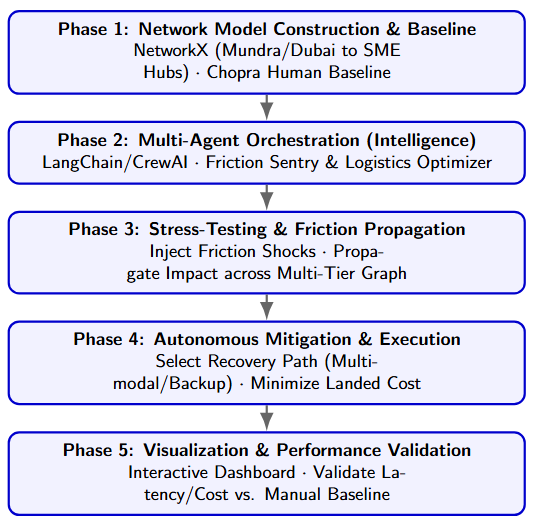
\includegraphics[width=0.65\textwidth]{Figures/methodology}
    \caption{Proposed methodology}
    \label{fig:methodology}
\end{figure}

\begin{itemize}
    \item \textbf{Phase 1: Network Model Construction \& Baseline Development:} A multi-tier logistics graph is developed using \texttt{NetworkX}, mapping critical nodes from international maritime chokepoints (e.g., Mundra, Dubai) to inland Indian SME clusters. A Manual Human Planner baseline is simultaneously established using Chopra inventory formulas to provide a performance benchmark for traditional, reactive supply chain management.
    \item \textbf{Phase 2: Multi-Agent Orchestration (Intelligence Layer):} Specialised autonomous agents are designed and deployed using \texttt{LangChain} and \texttt{CrewAI}. This includes a Friction Sentry for real-time monitoring of maritime signals (e.g., verification delays, insurance spikes, or congestion) and a Logistics Optimiser for executing autonomous rerouting and dynamic buffer-stock calculations.
    \item \textbf{Phase 3: Stress-Testing \& Friction Propagation:} One simulated Friction Shock---ranging from administrative bottlenecks to regional blockades---is injected into the graph model. The agents identify these disruption signals, propagate the impact across the multi-tier supply chain, and evaluate the mathematical trade-offs of various mitigation strategies.
    \item \textbf{Phase 4: Autonomous Mitigation \& Execution:} The agentic pipeline autonomously selects the most efficient recovery path, such as pivoting to multimodal transport or identifying backup suppliers, to minimise Total Landed Cost and operational downtime. This phase transitions the system from simple detection to executable action.
    \item \textbf{Phase 5: Visualisation \& Performance Validation:} The agentic output is integrated into an interactive Dashboard for real-time decision support. The framework's effectiveness is validated by comparing its response latency and cost-efficiency against the previously established manual baseline, targeting a measurable reduction in stockouts and overstocking.
\end{itemize}

\section[Expected Outcomes]{\textbf{Expected Outcomes}}
The expected outcomes of this project include:
\begin{itemize}
\item A functional multi-agent system using LangChain and CrewAI that transitions from passive monitoring to autonomous execution of mitigation strategies.
\item A dynamic NetworkX-based supply chain model integrated with a Tableau dashboard for real-time ``What-If'' scenario simulations and risk propagation visualisation.
\item A validated framework demonstrating reduced operational costs and stock-outs for Indian SMEs compared to traditional manual planning.
\end{itemize}

\section[Organisation of the Report]{\textbf{Organisation of the Report}}
The remainder of this report is organised as follows:

\begin{itemize}
    \item \textbf{Chapter 2 -- Theory and Fundamentals:} The theoretical foundations of Multi-Agent Systems, the Chopra inventory model, and the graph-theoretic principles used in the Logistics Digital Twin are discussed.
    \item \textbf{Chapter 3 -- Software Requirement Specification:} The detailed system requirements, functional specifications, and hardware/software prerequisites are defined.
    \item \textbf{Chapter 4 -- High-Level Design:} The architectural design, agent roles, and the integration of CrewAI with the NetworkX graph model are elaborated.
    \item \textbf{Chapter 5 -- Detailed Design:} The internal functional design, interaction protocols, and specific data structures used within the modular digital twin framework are focused upon.
    \item \textbf{Chapter 6 -- Implementation Details:} The coding standards, module connectivity, and the end-to-end integration of the backend services with the interactive dashboard are documented.
    \item \textbf{Chapter 7 -- Software Testing:} The verification of modules and system workflows through unit, integration, and performance benchmarking suites is presented.
    \item \textbf{Chapter 8 -- Results and Discussion:} The system's performance metrics are analysed and the agentic optimisation results are validated against human benchmarks.
    \item \textbf{Chapter 9 -- Conclusion and Future Scope:} The project's contributions are summarised, current limitations are identified, and a roadmap for future technical enhancements is proposed.
\end{itemize}

\section[Summary]{\textbf{Summary}}
This chapter introduced the project domain, problem statement, objectives, and the significance of the proposed work. The background of maritime logistics disruption, a comprehensive literature survey highlighting research gaps, the proposed methodology, and the expected outcomes of the project were discussed. The information presented in this chapter establishes the foundation for the detailed technical discussions provided in the subsequent chapters.
